\documentclass[11pt,UTF8]{ctexart}
\usepackage{titling}
\usepackage{enumerate}
\usepackage{amsmath}
\usepackage{amssymb}
\usepackage{amsfonts}
\usepackage{listings}
\usepackage{forest}
\usepackage{bm}
\usepackage{float}
\usepackage{graphicx}
\usepackage{multicol}
\usepackage{comment}
\usepackage[unicode=true,%本行非常重要 支持中文目录hyperref CJKbookmarks对二级目录没用
	colorlinks,
	linkcolor=black,
	anchorcolor=black,
	citecolor=black,
	CJKbookmarks=false]{hyperref}
\usepackage{xcolor}
\usepackage{geometry}
\geometry{top=20mm,bottom=20mm,left=20mm,right=20mm}
\pagestyle{plain}%删除页眉
\CTEXsetup[format={\Large\bfseries}]{section}

\setlength{\droptitle}{-50pt}%减少标题与页眉距离

\title{Project 3 实验报告\protect\footnote{\color{red}本文采用\LaTeX进行编写}}
\author{17341015 计一 陈鸿峥}
\date{}

\begin{document}
\maketitle
\vspace{-50pt}%减少标题与正文距离

\lstset{language=C++,escapechar=`}

\section{实验目的}
开发一个校园电子卡管理系统,可以实现以下三种电子卡的功能
\begin{itemize}
	\item 校园卡:\textbf{支付、查询}功能,需要注意
	\begin{enumerate}
		\item 不可透支
		\item 查询内容包括:
		\begin{itemize}
			\item 支出流水
			\item 转入流水
			\item 校园卡信息(学号、姓名、学院)
		\end{itemize}
		\item 只支持现金转入,不支持转出和提取
	\end{enumerate}
	\item 储蓄卡:\textbf{支付、查询、转账}功能,需要注意
	\begin{enumerate}
		\item 支付可以透支一定额度
		\item 查询内容包括:
		\begin{itemize}
			\item 支出流水
			\item 转账流水
			\item 储蓄卡信息(卡号、发卡日期、姓名)
		\end{itemize}
		\item 支持转出至三种不同的卡,支持提款,支持现金或其他储蓄卡转入
	\end{enumerate}
	\item 绑定卡:前两者的结合,但以校园卡功能为主,储蓄卡功能为辅
\end{itemize}


\section{实验环境}
\begin{enumerate}
	\item 系统环境:Windows 10
	\item 编程环境:Sublime Text 3
	\item 编程语言:C++
	\item 编译环境:gcc 6.3.0
\end{enumerate}


\section{实现思路}
校园电子卡管理系统的功能如下:
\begin{center}
\begin{forest}
for tree = {grow=east}
[校园电子卡管理系统
	[存储
		[读取]
		[存储]]
	[查询
		[卡信息]
		[卡流水]]
	[转账
		[提款]
		[转入]
		[转出]]
	[管理
		[添加卡类]
		[删除卡类]]]
\end{forest}
\end{center}


\section{设计细节}
\subsection{文件关系}
本多项式计算器包含六个源程序文件:
\begin{enumerate}
	\item \verb'main.cpp' 为主文件,包含上述四个模块及具体的交互界面
	\item \verb'card.hpp' 包含 \verb'card'基类,实现基础卡的功能
	\item \verb'campus_card.hpp' 包含 \verb'campus_card'类,继承 \verb'card'基类,并具有自己独特的功能
	\item \verb'deposit_card.hpp' 包含 \verb'deposit_card'类,继承 \verb'card'基类,并具有自己独特的功能
	\item \verb'binding_card.hpp' 包含 \verb'binding_card'类,继承 \verb'campus_card'和 \verb'deposit_card'类,并具有自己独特的功能
	\item \verb'card_repository.hpp' 包含 \verb'card_repository'类,即存储以上三种卡的仓库
\end{enumerate}
\par 具体依赖关系如下图所示.
\begin{figure}[H]
\centering
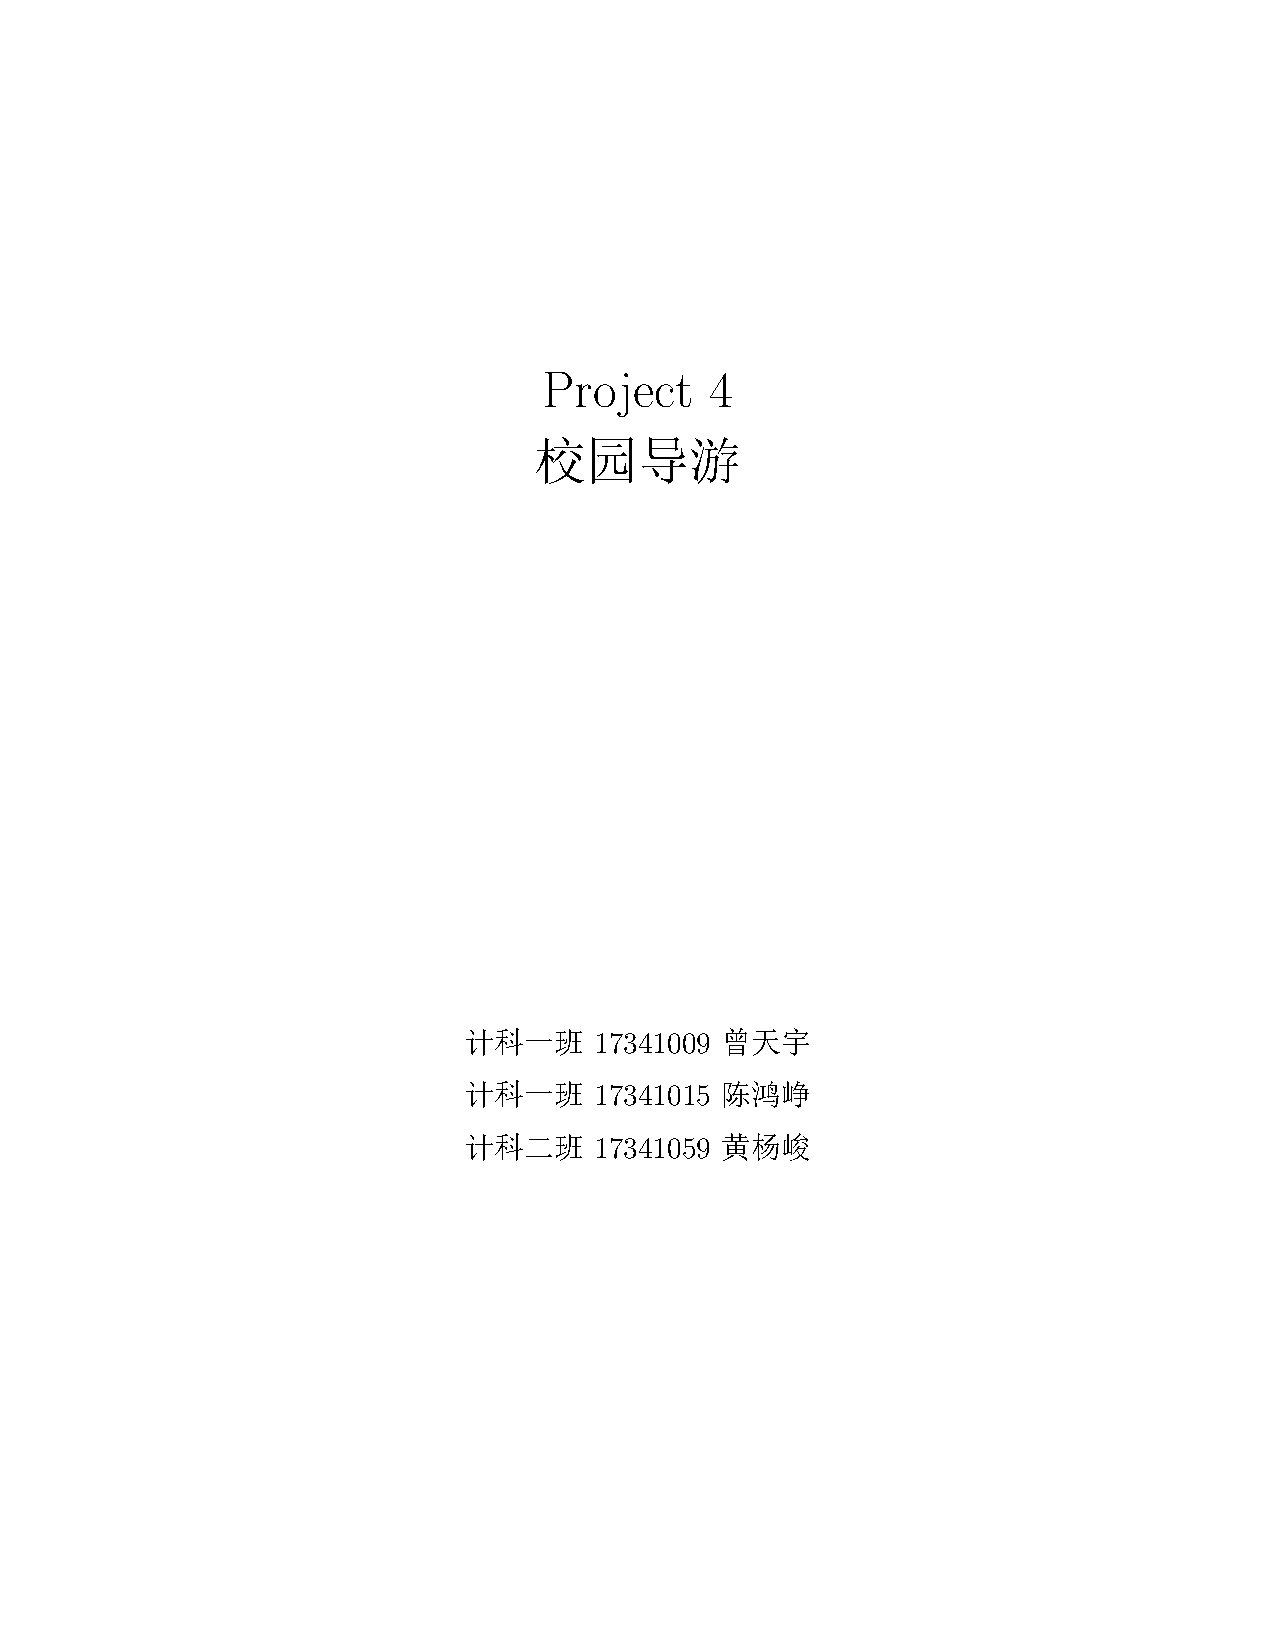
\includegraphics[width=\linewidth]{pic/main.png}
\end{figure}

\subsection{头文件}
\begin{enumerate}
	\item \verb'<string>',\verb'<vector>'为\verb'C++'标准库的容器,用于存储数据
	\item \verb'<iostream>',\verb'<fstream>'用于命令行及文件的输入输出
	\item \verb'<iomanip>'用于控制输出格式
	\item \verb'<regex>',\verb'<iterator>'为正则表达式和迭代器,用于字符串的分割
\end{enumerate}

\subsection{类结构设计}
\subsubsection{日期类}
\par 由于记录卡流水信息时需要用到日期,故先实现一个日期类,实际上为C的时间库\verb'<ctime>'的封装
\par 由于本校园卡系统是简单实现,故记录流水时只记录到日,而没有精确到时分秒
\begin{figure}[H]
\centering
\includegraphics[width=0.5\linewidth]{pic/Date_struct.PNG}
\end{figure}

\subsubsection{流水类}
\par 同样,记录卡的信息时需要记录流水,故直接开一个流水类,实现如下
\begin{figure}[H]
\centering
\includegraphics[width=0.6\linewidth]{pic/fr_struct.PNG}
\end{figure}

\subsubsection{卡基类}
\par 作为其他三类卡的基类,需要将大部分操作实现,具体实施细节如下
\par 由于基类的成员都需被继承,故设置为 \verb'protected'
\begin{figure}[H]
\centering
\includegraphics[width=\linewidth]{pic/card.PNG}
\end{figure}
\par 卡基类图示如下
\begin{figure}[H]
\centering
\includegraphics[width=0.8\linewidth]{pic/card_class.png}
\end{figure}
\par 以下三个类与卡基类的关系如图所示
\begin{figure}[H]
\centering
\includegraphics[width=0.4\linewidth]{pic/diamond.png}
\end{figure}

\subsubsection{校园卡类}
\par 继承 \verb'card'基类,注意是虚继承,因之后还会被继承一次,且是菱形继承;若不进行虚继承,会导致二义性错误
\begin{figure}[H]
\centering
\includegraphics[width=0.9\linewidth]{pic/campus_card.PNG}
\end{figure}
\par 校园卡类图示如下
\begin{figure}[H]
\centering
\includegraphics[width=0.8\linewidth]{pic/campus_card_class.png}
\end{figure}

\subsubsection{储蓄卡类}
\par 继承 \verb'card'基类,注意是虚继承,因之后还会被继承一次,且是菱形继承;若不进行虚继承,会导致二义性错误
\par 注意转账功能采用了泛型编程的思想
\begin{figure}[H]
\centering
\includegraphics[width=0.9\linewidth]{pic/deposit_card.PNG}
\end{figure}
\par 储蓄卡类图示如下
\begin{figure}[H]
\centering
\includegraphics[width=0.8\linewidth]{pic/deposit_card_class.PNG}
\end{figure}

\subsubsection{绑定卡类}
\par 继承 \verb'campus_card'和 \verb'deposit_card'类,同时将绑定的储蓄卡信息以指针的形式存入类成员中
\begin{figure}[H]
\centering
\includegraphics[width=0.9\linewidth]{pic/binding_card.PNG}
\end{figure}
\par 绑定卡类图示如下
\begin{figure}[H]
\centering
\includegraphics[width=0.8\linewidth]{pic/binding_card_class.png}
\end{figure}

\subsubsection{卡仓库类}
\par 统一存储三种卡,为主函数提供接口
\begin{figure}[H]
\centering
\includegraphics[width=0.9\linewidth]{pic/card_repository.PNG}
\end{figure}
\par 卡仓库类图示如下
\begin{figure}[H]
\centering
\includegraphics[width=0.6\linewidth]{pic/card_repository_class.PNG}
\end{figure}

\subsection{主函数设计}
\par 主函数中实现的函数如下,大多为交互界面的输入输出以及调用卡仓库类的接口
\begin{figure}[H]
\centering
\includegraphics[width=0.9\linewidth]{pic/main_function.PNG}
\end{figure}

\subsection{交互界面}
\par 由于交互界面实现代码过长,故不在此贴图,请到 \verb'main.cpp'中查看
\begin{figure}[H]
\centering
\includegraphics[width=\linewidth]{pic/interface.PNG}
\end{figure}
\begin{itemize}
	\item 用\verb'<iomanip>'控制输出格式确保美观
	\item 用\verb'cin.clear()'和\verb'cin.sync()'清空缓存区,确保每次输入被程序读入后不会有残留,避免干扰下一次操作
	\item 当字符串长度为$0$或大于$1$时循环读入字符串,避免读入空行或者错误输入
	\item 多重输入判定,对输入名字的合法性、名字是否与已有的卡冲突等进行判定,确保输入准确合法
\end{itemize}

\subsection{输入输出及存储}
\begin{enumerate}
	\item 输出可在命令行中手动输入,或者从文件流中直接读入
	\item 输出同时有命令行的输出和文件流的输出(但要选择保存),输出格式同输入
	\item 具体操作在交互界面均会提示,按照提示要求进行即可
\end{enumerate}
\par 由于存储的内容相似,故这里采用了泛型编程的思想,构造了一个模板,简化代码
\begin{figure}[H]
\centering
\includegraphics[width=0.9\linewidth]{pic/template.PNG}
\end{figure}

\par 存储会分别存在三个文档,\verb'Campus_card.dat'、\verb'Deposit_card.dat',\verb'Binding_card.dat'中,存储结构类似下图
\begin{figure}[H]
\centering
\includegraphics[width=0.4\linewidth]{pic/store.PNG}
\end{figure}
\par 第一行为一个数字$n$,代表该种卡有$n$张
\par 接下来一行会是第一张卡的信息,按顺序依次是卡号、开卡日期、姓名(学院)
\par 第三行是一个数字$m$,代表有$m$个流水数据
\par 流水数据依次按照日期、地点、变化金额、余额来记录
\par 如此往复,直到所有$n$条数据全部存储完毕
\par 对于绑定卡,则还会添加一行卡号,对应绑定的储蓄卡号码

\subsection{值得一提的细节}
\begin{enumerate}
	\item 代码符合C++11标准,尽可能在易读代码的同时简化代码
	\item 对于类的实施,一定会在必要的地方加上 \verb'const'和 \verb'inline'等关键词修饰
	\item 对于指针、引用的使用及其小心,尽可能避免多余、意外操作
\end{enumerate}


\section{程序测试及实验结果}
\par 添加卡类效果如下
\begin{figure}[H]
\centering
\includegraphics[width=0.6\linewidth]{pic/new_card.PNG}
\end{figure}
\par 转账功能如下
\begin{figure}[H]
\centering
\includegraphics[width=0.6\linewidth]{pic/transfer.PNG}
\end{figure}
\par 查询功能如下,可以见到若没有数据,也可以正常输出
\begin{figure}[H]
\centering
\includegraphics[width=0.6\linewidth]{pic/query.PNG}
\end{figure}
\par 实现了项目要求的所有功能,写了$1000+$行代码考虑了各种极端情况,确保程序足够鲁棒。以下是用到的一些\verb'C++11'特性:
\begin{enumerate}
	\item 利用泛型编程的思想,写模板函数,减少代码的重复
	\item \verb'split'函数在进行正则匹配时常常会导致程序崩溃:\\
		加上\verb'try,catch'特性捕获并避免发生异常
	\item 必要的地方都加上const限定,防止误操作修改类的私有数据
	\item 使用\verb'auto'自动推断类型
	\item 使用\verb'for'的范围语句简化代码
	\item 使用智能指针\verb'nullptr'
\end{enumerate}


\end{document}